% !TeX spellcheck = en_US
\section{Results}
		%------------------------------%
		%& 		References 				
		%------------------------------%  
	
		We report the means and standard deviations of \textit{p}-values of MvGLM, CQO, CCA, and dbRDA for all explanatory variables (Table \ref{table:results1::mean-p}), p-values for different response shapes and sample sizes are given in the Tables S 2 - 5.
		
		%------------------------------%
		%& Table: p-values + standard deviations
		%------------------------------% 

        \begin{table*}[ht]
            \centering
        	\caption{
        	    Mean \textit{p}-values $\pm$ standard deviations of the causal (env1 and env2) and noise variables from multivariate Generalized Linear Models (MvGLM), Constrained Quadratic Ordination (CQO), Canonical Correspondence Analysis (CCA), and distance-based Redundancy Analysis (dbRDA) for all models. 
        	    }
            \begin{tabular}{@{}
            >{\columncolor{white}[0pt][\tabcolsep]}
            cccc
            >{\columncolor{white}[\tabcolsep][0pt]} c
            @{}}
                \rowcolor{lightgray}
                & \textbf{MvGLM} & \textbf{CQO}      &  \textbf{CCA}     & \textbf{dbRDA} \\
                \toprule
                \textit{env1}  & $0.006 \pm 0.0275$   & $0.067 \pm 0.127$ & $0.264 \pm 0.433$ & $0.002 \pm 0.007$ \\
                \textit{env2}  & $0.009 \pm 0.0311$   & $0.090 \pm 0.190$ & $0.264 \pm 0.433$ & $0.003 \pm 0.011$ \\
                Noise          & $0.650 \pm 0.280$    & $0.680 \pm 0.268$ & $0.399 \pm 0.348$ & $0.523 \pm 0.256$ \\
                \bottomrule  
            \end{tabular}
            \label{table:results1::mean-p}	
        \end{table*}


	%------------------------------%
	%& 		GLMmv 					
	%------------------------------%
		%------------------------------%
		%& 			In General 			
		%------------------------------%
        In most MvGLMs, negative binomial residual distribution achieved the lowest AIC and the best fit to model assumptions. 
		%  
		The plot of Dunn-Smyth residuals against the linear predictor of \textit{LL} (Figure S 1) showed arched patterns, which could indicate that the residuals were not independent of the explanatory variables. 
        %
        Nevertheless, We used a negative binomial residual distribution because visual inspection of the QQ-Plots suggested that it resulted in a better fit than Poisson or Gaussian distributions. 

		%------------------------------%
		%& 	 p-values 	
		%------------------------------% 
		MvGLMs' \textit{p}-values for both causal variables and all response type combinations were low (Table  \ref{table:results1::mean-p}).
		%
        The \textit{p}-values of the linear variable in \textit{LB} and \textit{UL} and of the bimodal variable in \textit{UB} were higher at the smallest sample size than at higher ones (Table S 2).  
		%
		Otherwise, the samples size had no effect on the \textit{p}-values of the causal variables, which often were minimal (1 divided by the number of permutations + 1) at small sample sizes.
		%
		The \textit{p}-values for noise variables were higher and varied strongly (Figure \ref{fig:result1::p-valueComparison}).
		%
		They only fell below the nominal significance level of 0.05 in three models. 
		%
		All three models had the response combination \textit{LL} and the low \textit{p}-values occurred at the sample sizes 225, 625, and 900 (Table S 2).
		%
		%------------------------------%
		%& 	 FPR/ FNR  	
		%------------------------------%
		%
		The FPR was the lowest of all methods (0.008 at $\alpha = 0.05$) and always well below the respective significance level (Figure 3). 
		%
		Overall, FPRs and FNRs of MvGLMs were very low (Figure \ref{fig:FPNR}).
		%
        Interestingly the \textit{p}-values of noise variables did not show a monotonic positive relationship with samples size, as we expected. 
        %
        Rather the response seemed unimodal in \textit{UU}, \textit{LL}, and \textit{BB}, slightly negative in \textit{LB} and \textit{UL} and positive for \textit{UB} (Table S 2). \\ 
        
        \begin{figure}[h]
            \centering
            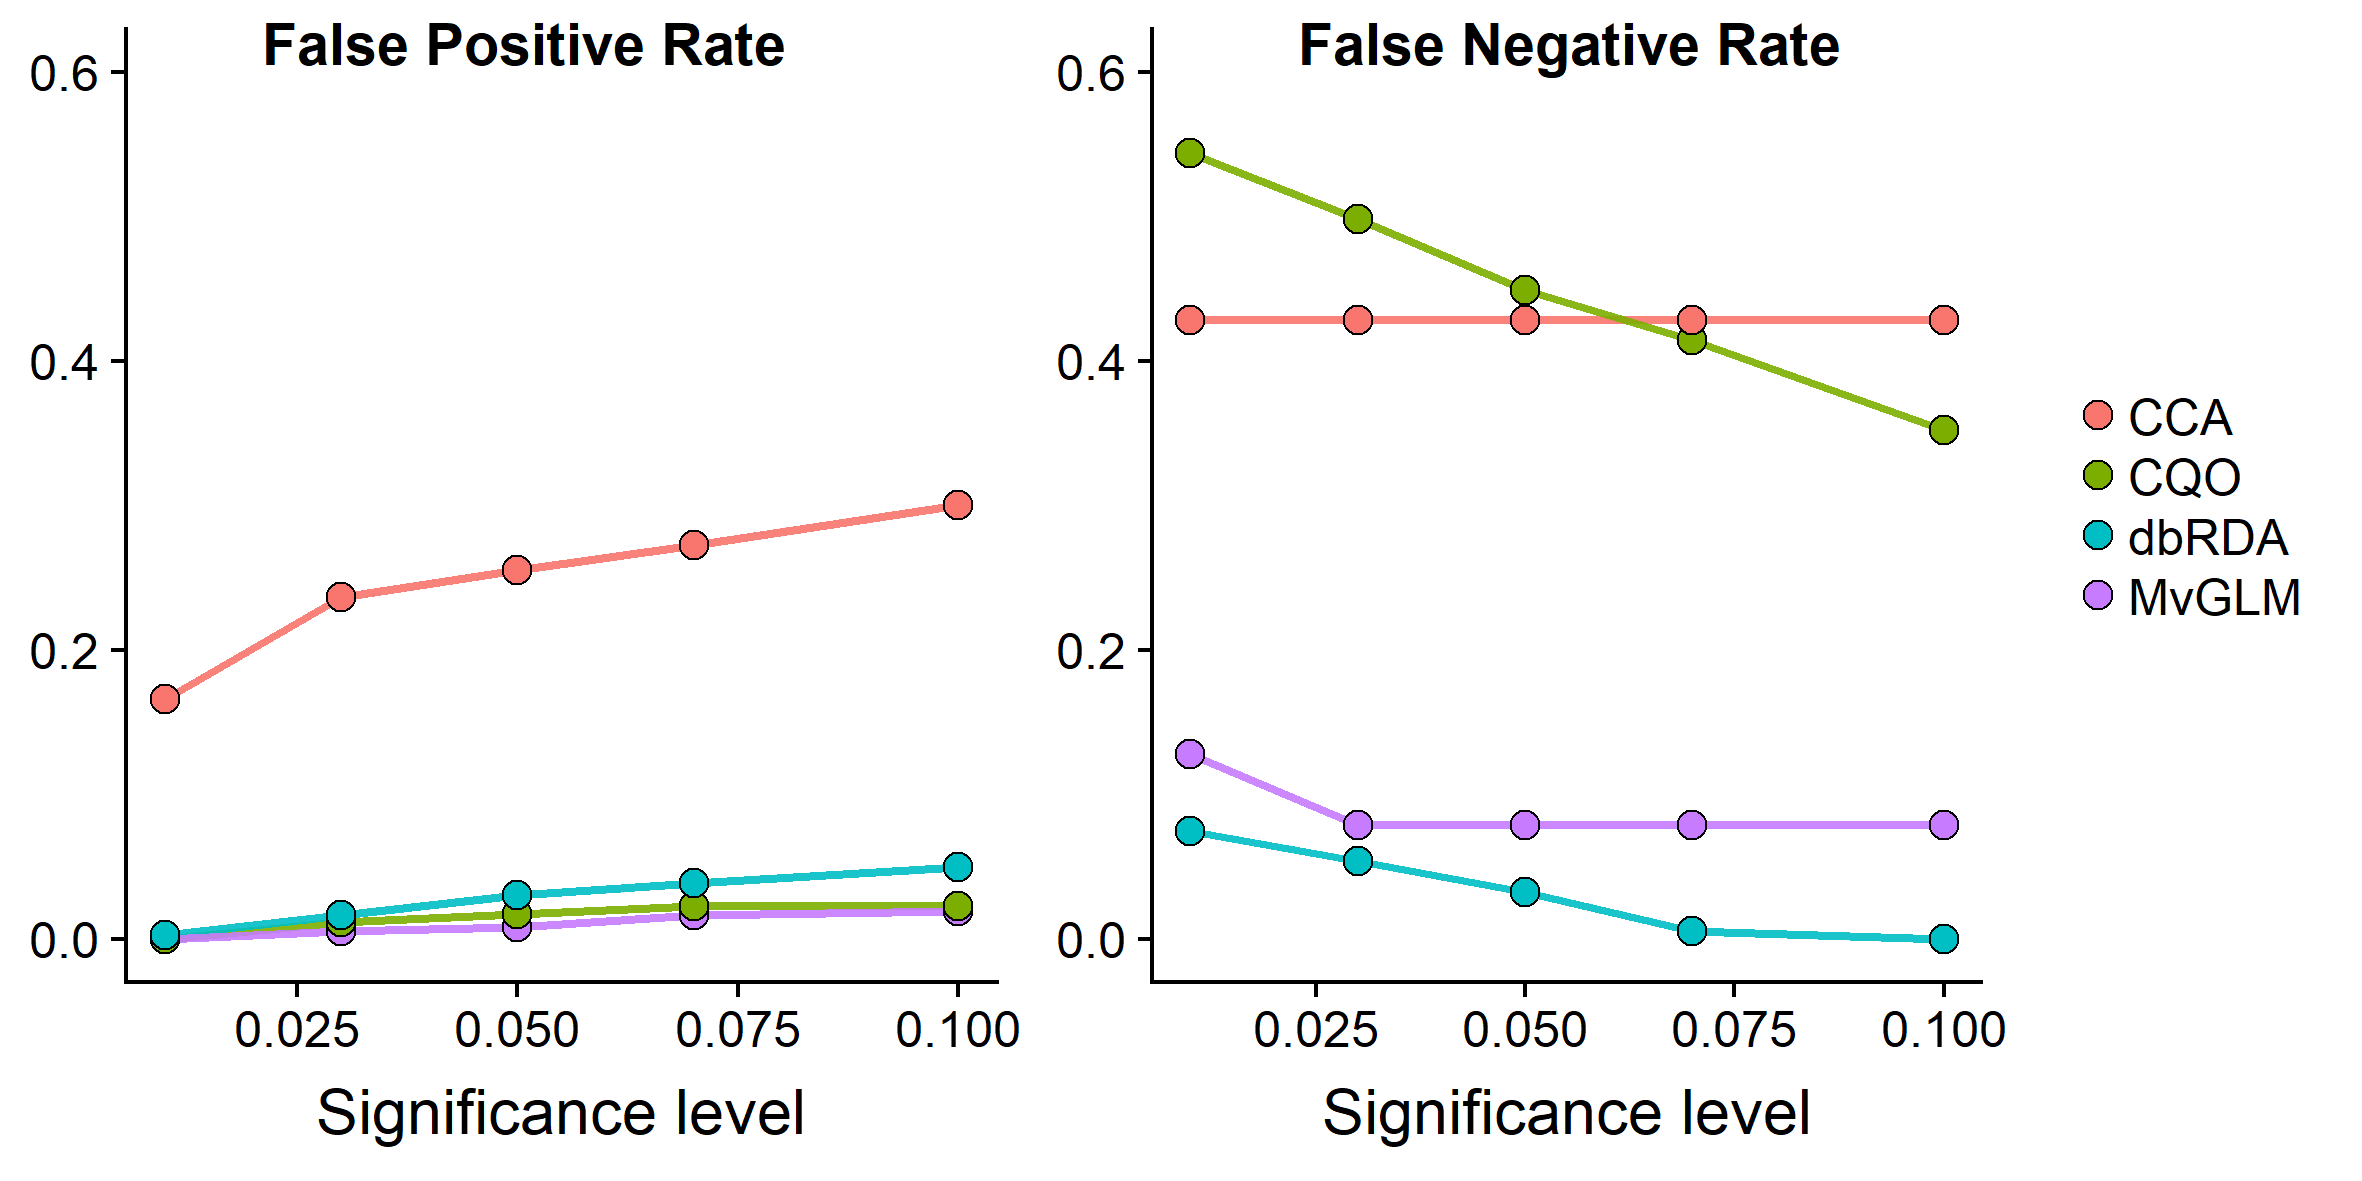
\includegraphics[scale = 0.7]{figures/FPNR.png}
            \caption{False Positive Rate and False Negative Rate of the four statistical methods Canonical Correspondence Analysis (CCA), Constrained Quadratic Ordination (CQO), distance based Redundancy Analysis (db-RDA), and multivariate Generalized Linear Model (MvGLM). }
            \label{fig:FPNR}
        \end{figure}{}
                    
    %------------------------------%
	%& 	CQO			
	%------------------------------% 
	
	CQOs performance strongly depended on the response shape (Figure \ref{fig:result1::p-valueComparison}). 
    %
    It failed to converge for \textit{UB} with sample size 25 and performed best for \textit{UU} and \textit{BB}; both had a FNR of 0 FPRs below the average (0 and 0.06 respectively).
    %
    \textit{UB} performed slightly worse than \textit{UU} and \textit{BB} with an FNR of 0.1 and an FPR of 0.02.
	%
	As was expected, CQO often assigned high \textit{p}-values to linear causal variables (Figure \ref{fig:result1::p-valueComparison}). 
	%
	The mean \textit{p}-value of linear variables was 0.15 and their FNR was 0.53. 
	%
	Both unimodal and bimodal causal variables received higher \textit{p}-values when the other causal variable was linear (Table S 3).
	%
	The mean \textit{p}-value of unimodal variables excluding those from \textit{UL} is $0.006\pm0.022$ compared to $0.036\pm0.084$ for the unimodal variable in \textit{UL}.
	%
	Similarly, the mean \textit{p}-value of bimodal variables except for those form \textit{LB} is $0.004\pm0.015$ and for the bimodal variable in \textit{LB} it is $0.042\pm0.083$.
	%
    This mixed performance leads to relatively high mean \textit{p}-values for the causal variables (Table \ref{table:results1::mean-p}) and accordingly high FNR and FPR (Figure \ref{fig:FPNR}).\\
    
    \begin{figure}
        \centering
        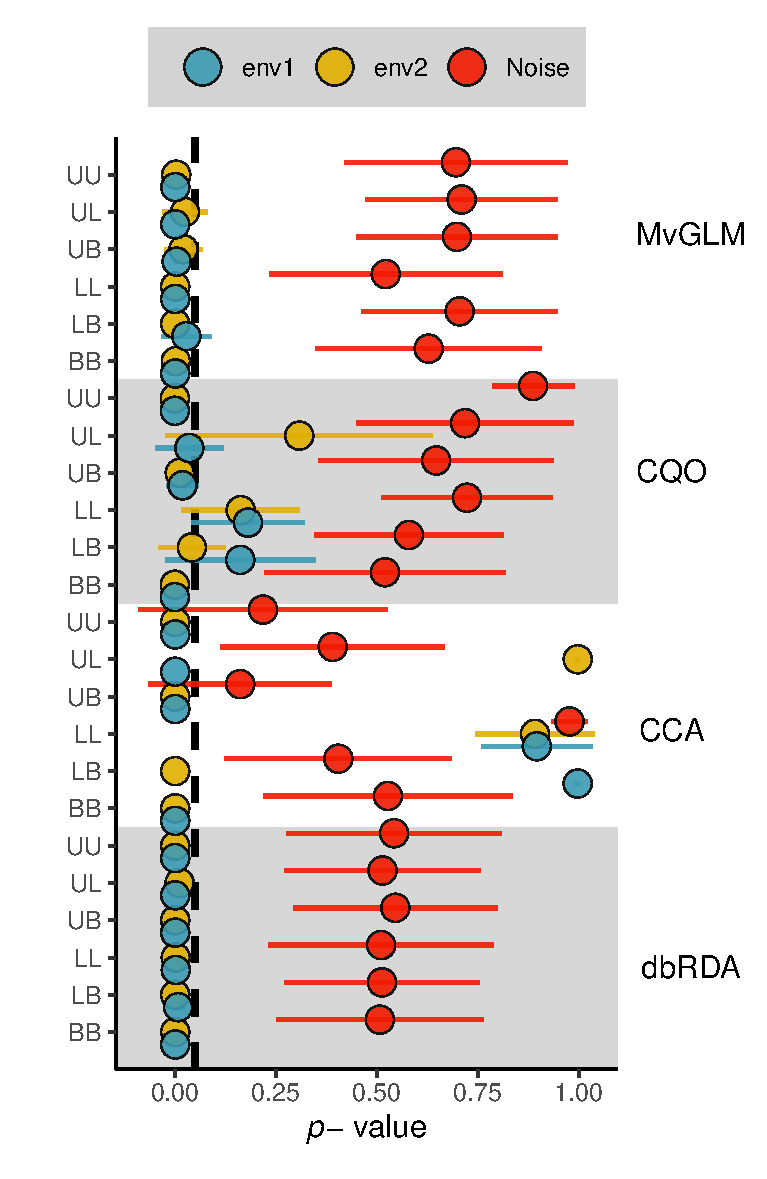
\includegraphics[scale = 0.7]{figures/190912_error_bar.pdf}
        \caption{Mean \textit{p}-values of response combinations (indicated by first letter of response types: unimodal (U), linear (L), bimodal (B)) for multivariate Generalized Linear Models (MvGLM), Constrained Quadratic Ordination (CQO), Canonical Correspondence Analysis (CCA), and distance-based Redundancy Analysis (dbRDA). Blue points are \textit{env1}, yellow points \textit{env2} and red points are noise variables. Bars shows one standard deviation. The vertical, dashed line indicates a \textit{p}-value of 0.05.}
        \label{fig:result1::p-valueComparison}
    \end{figure}
    %------------------------------%
	%& 			CCA					
	%------------------------------% 

		%------------------------------%
		%& 			Variables			
		%------------------------------% 

		CCA has the highest mean \textit{p}-values for causal variables and the lowest for noise ones. 
		%
		Accordingly, the FPR was the highest of all methods (Figure \ref{fig:FPNR}.
		%
		Irrespective of significance level, it is more than one order of magnitude higher than for all other methods.
		%
		These problems are due to two factors: i) high \textit{p}-values for causal linear variables and ii) low \textit{p}-values for noise variables. 
		%
		The mean \textit{p}-value for causal linear variables is $0.963\pm0.094$. 
		%
        Additionally, CCAs of \textit{LL} with sample sizes 400 to 900 produced constrained inertias (explained variance) of 0 and were therefore excluded from significance testing. 
		%
		Noise variable \textit{p}-values were especially low in \textit{UU} and \textit{UB} (Figure \ref{fig:result1::p-valueComparison}), which is interesting since these data sets matched closest with the assumed \textit{species packing model}.  
		%
		In \textit{BB} they were markedly higher (Table S 4). 
		%
        The impact of different sample sizes was negligible in all response combinations (Table S 4).   

	%------------------------------%
	%& 	db-RDA 	
	%------------------------------%

		The dbRDA assigned low \textit{p}-values to most causal variables (Figure \ref{fig:result1::p-valueComparison}).
		%
		The only \textit{p}-values of causal variables above the nominal significance level of 0.05 were those of linear variables at a sample size of 25 (Table S 5).
		%
		However, they were below 0.1, so that the dbRDA had an FNR of 0 at $\alpha = 0.1$.  
		%
		Indeed, the FNR was the lowest of all methods (Figure \ref{fig:FPNR}).
		%
        The \textit{p}-values were relatively similar for all sample sizes (Table S 5). 
		%
        The FPR of dbRDA was relatively high, with 0.031 at $\alpha = 0.05$.  
        %
        The FNR was the lowest of all methods. \\
        %
        Both algorithm-based methods were considerably faster than the model-based ones (Figure S 2).

	